\documentclass[a4paper, 12pt]{article}
\usepackage[brazil]{babel}
\usepackage[utf8]{inputenc}
\usepackage[T1]{fontenc}
\usepackage{ae}
\usepackage{sbc-template}
\usepackage{url}
\usepackage{booktabs}
\usepackage{listings}
\usepackage{float}
\usepackage{paralist}
\usepackage{clrscode3e}
\usepackage{graphicx}

\title{Aplicação das metaheurísticas de Otimização por Colonia
de Formigas e Algoritmos Meméticos para o Problema de Atribuição Quadrático}
% sugestão :p Nao vai dar tempo de fazer um "estudo comparativo"

\author{Guilherme Polo\inst{1}, Maycon Sambinelli\inst{1}}

\address{Departamento de Informática -- Universidade Estadual de
  Maringá (UEM)\\
  CEP -- 87020-900 -- Maringá -- PR -- Brazil
\email{\{ggpolo,msambinelli\}@gmail.com}
}

\begin{document}

\maketitle

\begin{abstract}
Empty abstract.
\end{abstract}

\begin{resumo}
Resumo vazio.
\end{resumo}

\section{Introdução}

O PQA (Problema Quadrático de Atribuição/Alocação), ou QAP (
\textit{Quadratic Assignment Problem}) \cite{qap-origin} é um dos
mais conhecidos e difíceis problemas de otimização combinatória
\cite{Maniezzo98exactand}. Entre suas aplicações, \cite{QAPBOOK} cita:
problemas de localização de instalações, escalonamento, problemas de
fiação em eletrônica, computação paralela e distribuída \cite{22},
analise estatística de dados, projeto de painéis de controle e teclados,
química, arqueologia, balanceamento de rotores de turbinas e
manufatura de computadores.
% Em \cite{hospital} é abordado um problema real onde 30
% instalações (\textit{facilities}) eram associadas a 30 locais no
% hospital universitário Klinikum
% Regensburg na Alemanha, problema este que é conhecido hoje como {\it
% Kra30a}, desde que foi incluído na QAPLIB.

%Coisas a arrumar no parágrafo anterior: \\
%XXX A QAPLIB fala de uma publicação de 1978 sobre os problemas do krarup, por
%que tem esse artigo de 2000 aqui ? XXX
%XXX Não tinha sido dito nada da QAPLIB até agora, ficou estranho
%colocar o nome dela no final do paragráfo XXX

Solucionar um QAP consiste em encontrar a melhor alocação de $n$
instalações para $n$ localizações. Matematicamente o problema pode ser
formulado como o de minimizar a seguinte função:
\begin{equation}\label{calc-custo}
C(\pi) = \sum_{i = 1}^{n} \sum_{j = 1}^{n} f_{ij} d_{\pi(i)
   \pi(j)} \, , \quad \pi \in \prod(n)
\end{equation}
dadas duas matrizes, $F$ e $D$, de ordem $n \times n$, onde $\prod(n)$ é o
conjunto de todas as permutações de $\{1, \ldots , n\}$.

Devido a sua dificuldade, trabalhos publicados têm historicamente
notificado a solução exata de instâncias do QAP somente para valores
pequenos de $n$, com este variando entre
10 \cite{qap-origin} e 30 \cite{stutzle04}.
Por esse motivo, diversos métodos heurísticos têm sido propostos
para o QAP de modo a rapidamente produzir resultados aceitáveis.

Neste trabalho, a abordagem ao problema ocorre com uso de duas
metaheurísticas: \begin{inparaenum}[(1)] \item Otimização por Colônia
  de Formigas, ou {\it Ant Colony Optimization} (ACO) \cite{ACO}, que é
uma heurística inspirada no comportamento das formigas;
\item Algoritmo Memético (AM), ou \textit{Memetic Algorithm}\cite{moscato1},
que opera baseado em uma população e tenta imitar a evolução
cultural\end{inparaenum}.

Este artigo foi dividido em três seções (além desta introdução). Na
sequência é fornecido um embasamento teórico que visa esclarecer
termos mencionados ao longo do trabalho. Depois discute-se as
implementações realizadas e finalmente os resultados obtidos são
apresentados.

XXX No parágrafo anterior, falar sobre os resultados obtidos


\section{Fundamentação teórica}
\label{sec:fund}

O QAP é um problema de otimização classificado como
$\mathcal{NP}$--difícil,
portanto desconhece-se um algoritmo de tempo polinomial que resolve
este problema. Aproximações ($\epsilon-approximation$), para qualquer
instância, para este problema também foram classificadas como
$\mathcal{NP}$--difícil \cite{sahni-gonzales}.
% XXX Também tem um trabalho que trata de busca local com custo
% exponencial em QAP.

Há pelo menos duas formas de definir a função objetivo deste problema.
A Equação \ref{calc-custo} apresenta uma primeira forma,
mas também é comum encontrar a seguinte formulação:
\begin{equation}\label{calc-custo2}
C(\pi) = \sum_{i = 1}^{n} \sum_{j = 1}^{n} f_{ij} d_{\pi(i)
   \pi(j)} + \sum_{i = 1}^{n} a_{\pi(i) i} \, , \quad \pi \in \prod(n)
\end{equation}
onde a matriz A apresenta valores $a_{ij}$ que indicam o custo de
colocar a instalação $i$ na localização $j$. A Equação
\ref{calc-custo2} descreve o problema denominado de QAP generalizado
de Koopmans--Beckmann. % XXX Citar talvez
Nos dois casos, a matriz $F$ é chamada de matriz de fluxos, onde
$f_{ij}$ representa o
fluxo de material da instalação $i$ para a $j$. A matriz $D$ é chamada
de matriz de distâncias, com $d_{kl}$ representando a distância da
localização $k$ a $l$.% Alguns autores trazem também uma matriz $C$,
%que realiza associação de custos, mas costuma ser ignorada por não
%trazer contribuição significante para a complexidade do  problema
%\cite{QACO}.

% XXX Ficou na parte de implementação puramente aleatória, talvez
% trazer pra cá.
%Falar de como uma solução é representada neste trabalho.


Falar de como detectar instâncias díficies da QAP! Usando flow
dominance e distance dominance!


Falar do custo de utilizar métodos para solução exata e
por isso formas alternativas tem sido utilizadas.
Falar que utilizou metaheurísticas e juntar com o parágrafo seguinte

% XXX Peguei do meu outro trabalho esse primeiro parágrafo.
% Mudar, complementar, etc.
De acordo com \cite{metatheory}, metaheurísticas são uma
classe de métodos aproximativos projetados para atacar problemas
difíceis de otimização combinatória que não obtiveram sucesso por meio
de heurísticas clássicas. Pode-se dizer que metaheurísticas são
heurísticas que guiam heurísticas, de modo que sejam combinados
conceitos diversos para exploração do espaço de busca permitindo a
fuga de ótimos locais.

Falar que o trabalhou utilizou ACO e AM, que são apresentados nas
Subseções seguintes.

\subsection{Heurística Melhorativa}
% XXX Começo é praticamente o que tinha no meu outro trabalho

Partindo de uma solução factível, é possível reduzir seu custo por
meio de uma heurística melhorativa. Um ótimo local pode ser obtido com
esse tipo de heurística. O ótimo global pode coincidir com o custo do
caminho final encontrado, mas esse método não fornece meios de se
asserir esta informação.

De acordo com \cite{gutin-punnen}, o método utilizado neste trabalho é
classificado como ``método de transição de vizinhança'' pois são
procedimentos de busca local que movem de uma solução a outra baseados
na estrutura da vizinhança. Em geral, diversas iterações ocorrem até
que se chegue ao ótimo local.

Para a busca local com troca de pares (\textit{pairwise interchange}),
cada iteração encontra e realiza, se houver, a melhor troca de duas
instalações quaisquer (Figura \ref{fig:localstep}).
O procedimento é encerrado quando não for possível realizar nenhuma
troca.

\begin{figure}
  \centering
  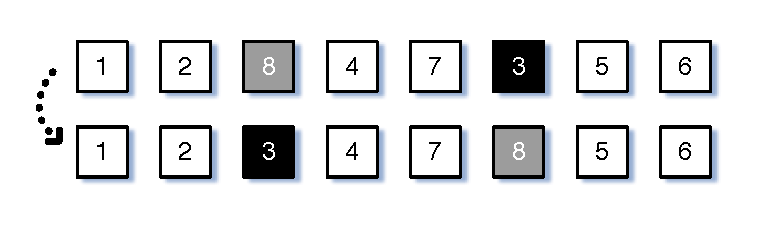
\includegraphics[scale=0.65]{pairchange}
  \caption{Uma troca, entre 8 e 3, na busca local\label{fig:localstep}}
\end{figure}

Após uma troca, para identificar o novo custo da solução sem recorrer
a Equação \ref{calc-custo}, ... XXX

\subsection{Otimização por Colônia de Formigas}

Otimização por Colônia de Formiga foi proposto originalmente por Dorigo em
\cite{aco-origin}. A meta-heurística ACO define uma classe de algoritmos
de formiga. Algoritmos de formiga são sistema multi-agentes no qual o
comportamento de cada agente ~\cite{aco-origin2}, chamado formiga artificial
ou apenas formiga, é inspirado no comportamento real das formigas biológicas.
A inspiração de desenvolver um algoritmo que simule o comportamento de uma
colônia de formigas, se deu após o experimento de Goss et. al.\cite{Goss}.

Em seu experimento, Goss utilizou uma colonia de formigas argentinas ({\it
Iridomyrmex humilis}). Entre a colonia de formigas e a fonte de comida, Goss
colocou uma ponte que se ramifica em dois caminhos, como ilustra a Figura
~\ref{fig:ponte}, fazendo com que uma formiga tenha que escolher uma das
ramificações. Após um momento inicial, foi observado que a maioria das
formigas passavam a escolher o menor caminho entre a colonia de formigas
e a fonte de comida. Esse comportamento ocorre devido a uma comunicação
indireta entre as formigas, que funciona como um mecanismo de{\it feedback}
positivo. Quando uma formiga caminha por um determinado caminho, ela deposita
no chão uma substância química chamada feromônio. Quando uma formiga
chega em um ponto de decisão, como a ramificação da ponte, ela faz uma
decisão probabilística baseada na quantidade de feromônio encontrada
nas ramificações. Essa decisão leva a um efeito de autocatálise pois
ao fazer a decisão de um caminho a seguir a formiga reforça ainda mais a
quantidade de feromônio naquele caminho o que aumenta a probabilidade desse
caminho ser escolhido por futuras formigas.

Inspirado no trabalho de Goos, Colorni desenvolveu o primeiro algoritmo
baseado em colonia de formigas o {\it Ant System} (AS) ~\cite{as-origin}.
No AS as formigas caminham em um grafo de componentes de soluções $C$,
adicionando componentes de solução a uma solução passo a passo. Para
determinar se uma componente deve ser adiciona a solução, cada formiga
faz uma decisão aleatória, baseada na quantidade de feromônio e
na informação heurística associada aquela componente. Para associar um
quantidade de feromônio a uma solução é utilizada uma matriz de feromônio
$T_{ij}$, onde cada elemento $\tau_{ij}$ representa a quantidade de feromônio
associada componente $c_{ij}$. No final de cada iteração, todas as formigas
atualizam essa matriz de feromônio, baseada nas suas respectivas soluções.

Inspirado no AS, Hoos \cite{mmas-origin} propôs um melhoramento chamado
$\mathcal{Min-Max}$ Ant System ($\mathcal{MMax}$). Sua principal intenção
era evitar a estagnação precoce, o que faz com que todas as formigas sigam
sempre o mesmo caminho e parem de explorar o espaço de busca. Como principal
modificação para atingir esse objetivo, o $\mathcal{MMax}$ delimita um
intervalo para o feromônio $\tau_{min} \le \tau_{ij} \le \tau_{max}$,
e assim evita que uma componente de solução acumule muito feromônio, % xxx melhorar isso
o que levaria as formigas a sempre escolherem ela.

\subsection{Algoritmos Meméticos}

Algoritmos Meméticos \cite{moscato1} são metaheurísticas baseadas
em população e evolução cultural.
Seu nome é derivado do termo \textit{meme} \cite{dawkins}, que é
definido por \cite{oxford-dict} como um elemento cultural que consegue
replicar-se por meios não-genéticos, como a imitação.
%an element of a culture or system of behaviour that may be considered
%to replicate by passing from one individual to another by nongenetic
%means, esp. imitation (página 271 do dicionário)
O trabalho de \cite{moscato1} faz uma comparação entre algoritmos
meméticos e artes marciais, tratando os movimentos coordenados e
eficazes dos mestres do Kung-Fu como algo que foi sendo aperfeiçoado
a partir do conhecimento formado por cada mestre. Este mesmo trabalho
também menciona que:
\begin{quote}
\textit{``A scientist does not pass on an idea after blending it with
  his own without checking the logic of what he is saying or his
  reputation would be in trouble. Altough there are some
  exceptions, science does not improve by random errors.''}
\end{quote}
Com estas analogias à AM deve ser possível observar que a mutação, ao
contrário de algoritmos genéticos (AG), não é um operador
característico desta metaheurística.
% XXX Colocar em algum lugar que AM também é conhecido como genético
% híbrido

Neste método, uma população (um conjunto de soluções, ou cromossomos
em AG, factíveis) é
inicialmente criada. Cada indivíduo (uma solução factível) é um ótimo
local. A cada geração (iteração) trabalha-se com recombinações,
seguido de obtenção de ótimo local, de indivíduos da população
atual. O operador de mutação é utilizado no caso de uma
geração apresentar baixa diversidade, ou seja: os indivíduos estão
mais semelhantes que um valor limite estabelecido.
%geração apresentar baixa diversidade, ou seja: os alelos ..  genes
%(elementos que compõem uma solução) na população estão
%suficientemente parecidos. XXX muita notação à toa..
Ao estabelecer um limite para o tamanho do conjunto de soluções,
torna-se necessário o uso de uma função que seleciona os indivíduos
mais adaptados dos demais para permanecerem na população.


\section{Implementação}

\subsection{Puramente aleatória}

A obtenção de soluções de instâncias do QAP por meio de um algoritmo
puramente aleatório é simples. Apesar desta forma de resolução não
fazer parte na coleta de resultados, ela é útil na discussão a
respeito da representação de soluções e custos envolvidos.

\begin{codebox}
\Procname{$\proc{qap-random}(F, D)$}
\li $\id{melhor-sol} \gets \emptyset$
\li $\id{melhor-custo} \gets \infty$
\li \While critérios de parada não satisfeitos \Do \label{criterio-random}
\li     $\id{sol} \gets \proc{solução-aleatória}()$
\li	$\id{custo} \gets \proc{calc-custo}(F, D, \id{sol})$
\li	\If $\id{custo} < \id{melhor-custo}$ \Then
\li		$\id{melhor-custo} \gets \id{custo}$
\li		$\id{melhor-sol} \gets \id{sol}$
        \End
    \End
\li \Return ($\id{melhor-sol}, \id{melhor-custo}$)
\end{codebox}

A função \proc{qap-random} recebe as duas matrizes que descrevem uma
instância QAP e retorna a melhor solução, com seu respectivo custo,
encontrada. Se implementado, critérios de parada (linha
\ref{criterio-random}) podem ser quantidade de iterações ou quantidade
de iterações sem redução de custo. Uma solução é construída com uso da
função \proc{solução-aleatória}, sendo esta também utilizada em certos
momentos das metaheurísticas desenvolvidas aqui. Calcular o custo de
cada solução envolve o uso da Equação \ref{calc-custo}, cuja
complexidade computacional é $\Theta(n^2)$. Logo, para ser
compatível com esta equação, uma solução precisa ser uma das $n!$
permutações possíveis para uma instância com matrizes de ordem
$n \times n$.

Representar uma solução qualquer na forma de permutação, como por
exemplo: $[1\,\, 4\,\, 2\,\, 3]$, tem o significado de atribuir a
instalação 1 na localização 1, instalação 4 na localização 2 e assim
por diante. De forma geral, a instalação $\pi(i)$ fica
localizada em $i$. Esta é uma forma simples de representar soluções no
QAP, sendo necessário cuidados para evitar o custo da Equação
\ref{calc-custo} caso a solução seja modificada em métodos de busca
local, mas foi utilizada ao longo deste trabalho.

\subsection{ACO}

\subsection{AM}

A forma geral do AM desenvolvido é:

\begin{codebox}
\Procname{$\proc{qap-memético}(F, D)$}
\li $\id{pop} \gets \proc{população-inicial}(F, D)$ \label{popinit}
\li \While critérios de parada não satisfeitos \Do \label{am-criterios}
\li     \For $i \gets 1$ \To $\const{n-recomb}$ \Do
\li	    $r \gets \proc{recombinar}(\proc{random-select}(pop, 2))$
\li	    $\proc{insere-ordenado}(pop, \proc{busca-local}(F, D, r))$
	\End
\li	\If $\proc{convergiu(pop)}$ \Then
\li	    $\proc{mutacionar}(pop[2:])$ \label{am-mutate}
	\End
\li     \If $\proc{estagnou}()$ \Then
\li         $\id{pop} \gets \id{pop}[1] \cup \proc{população-inicial}(F, D)$
        \End
    \End
\li \Return $\id{pop}[1]$
\end{codebox}

A população inicial, linha \ref{popinit}, é criada de forma puramente
aleatória, mas a
\proc{busca-local} é utilizada em todos os indivíduos gerados. Essa
população é mantida em ordem crescente de custo, de modo que a
primeira ali contida ($\id{pop}[1]$) sempre indique a melhor solução
encontrada. O tamanho desta população é variável, atualmente iniciando
com um valor um pouco abaixo do máximo permitido.

Como critérios de paradas, linha \ref{am-criterios}, são aceitos:
quantidade de gerações, tempo máximo de execução, valor atingido. Essa
última refere-se a especificação de um valor a ser alcançado, ao
término de uma geração é verificado se a melhor solução é menor ou
igual a esse valor e encerra, ou não, a execução.

Para realizar as recombinações, um parâmetro $\const{n-recomb}$ é
estabelecido e indica a quantidade destas a serem feitas. A função
$\proc{random-select}$ tem o cuidado de escolher dois indivíduos
distintos da população para cada recombinação. Em seguida,
$\proc{insere-ordenado}$ preocupa-se em manter a população ordenada ao
inserir o novo indivíduo gerado a partir da recombinação seguido de busca
local. Dois detalhes estão envolvidos nesta operação de
inserção: \begin{inparaenum}[(1)] \item a
variável $\id{pop}$ é tratada como um conjunto, portanto
soluções já existentes são descartadas; \item um novo indivíduo é
inserido na população somente se esta já não estiver em seu tamanho
limite ou se o mesmo não for pior que o pior atual\end{inparaenum}. O
operador de recombinação (função \proc{recombinar}) foi implementado
de forma bastante semelhante com aquele descrito em
\cite{merz_freisleben} e a Figura \ref{fig:recomb-op} demonstra seu
funcionamento.

\begin{figure}
  \centering
  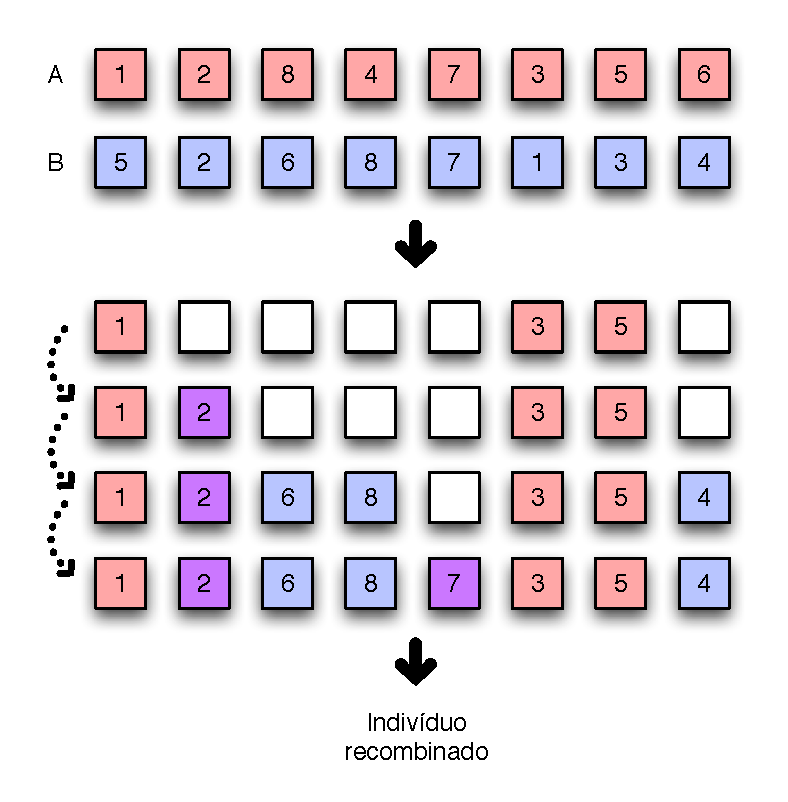
\includegraphics[scale=0.67]{recomb-op}
  \caption{Exemplo de recombinação realizada entre dois
    indivíduos\label{fig:recomb-op}}
\end{figure}

Na Figura \ref{fig:recomb-op}, as soluções \verb!A! e \verb!B! foram
escolhidas para serem recombinadas. A função \proc{recombinar} passa
por todas as posições, da esquerda para a direita, destes
indivíduos. Logo na primeira posição, a função encontra os valores 1 e
5. Por serem diferentes, aleatoriamente escolhe-se entre copiar um dos
valores para o resultado final. No exemplo, o valor 1 foi
copiado. Depois de realizar essa cópia, o seguinte processo é feito
para garantir que não haja mutações: \begin{inparaenum}[(1)] \item
  verifica se o elemento não copiado faz parte do resultado; \item
  caso não faça, encontra-se a respectiva posição em \verb!A! do
  mesmo; \item copia este valor na mesma posição no resultado
  final; \item elemento não copiado passa a ser o da posição atual de
  \verb!A!; \item volta para o primeiro passo enquanto este elemento
  não copiado não fizer parte da solução\end{inparaenum}.
Com isso, os valores 5 e 3 são copiados antes do elemento não copiado
tornar-se o valor 1 que já faz parte da solução. Um processo análogo é
feito quando seleciona-se um valor de \verb!B! para ser
copiado. Seguindo na passagem da esquerda para direita,
\proc{recombinar} encontra o valor 2 nos dois indivíduos e portanto
apenas copia o mesmo para o resultado. Na próxima posição escolhe-se o
valor 6 de \verb!B! para ser copiado, ocasionando também a inserção de
8 e depois 4. Avançando mais uma posição, o algoritmo encontra que a
mesma já foi preenchida com algum valor e não faz nada. Os demais
passos repetem o que já foi descrito.

Quando a busca local por troca de pares é aplicada a um indivíduo
recombinado, é feito uso de informações exemplificadas na Figura
\ref{fig:recomb-op}. Posições onde \verb!A! e \verb!B! contém o
mesmo valor não são utilizadas nas trocas, ficando fixas. Isso reduz o
número total de trocas nestes casos e, ao mesmo tempo, faz com que o
indivíduo resultante siga o propósito dos algoritmos meméticos:
se duas soluções encontraram a mesma localização para uma mesma
instalação, então repassar essa informação é um meio de permitir focar
na evolução de outras partes do problema.

Internamente é mantido uma variável que identifica se a população foi
modificada por meio de recombinações ou não. Caso os elementos
produzidos com este operador não apresentem nada diferente para a
população, um contador é incrementado; caso contrário este mesmo
contador é definido em 0. Isso é utilizado como um critério de
convergência. O outro critério é calculado, em todas as gerações, da
seguinte forma:
\begin{equation}\label{D}
D = \frac{\sum\limits_{i = 1}^{|pop|} \sum\limits_{j = i + 1}^{|pop|} dist(pop[i],
  pop[j])}{\frac{|pop| (|pop| - 1)}{2}}
\end{equation}
onde $dist$ retorna a quantidade de posições, em duas soluções, que
não possuem o mesmo valor; na Figura \ref{fig:recomb-op} isso ocorre
nas posições 1, 3, 4, 6, 7, 8 e portanto $dist(A, B) = 6$. O valor
retornado por $|pop|$ é o tamanho atual da população. Com isso, caso o
valor de $D$ fique abaixo de um limite, ou o outro critério seja
satisfeito, o operador de mutação, linha \ref{am-mutate} de
\proc{qap-memético}, é utilizado.

Na mutação preserva-se somente a melhor solução, indicado pela notação
de \textit{slice} (tomado da linguagem de programação \texttt{Python})
na linha \ref{am-mutate}. Um detalhe de implementação é que o pior
elemento também é preservado, diferindo um pouco do método descrito em
\cite{merz_freisleben}, de modo a tentar diversificar um pouco mais a
população. A implementação deste operador baseia-se no tamanho da
instância e também no valor limiar,
que decide se $D$, da Equação \ref{D}, é baixo ou não, para definir o
quão modificado será cada indivíduo. Atualmente o limiar é calculado
como: $\lfloor\frac{n}{2}\rfloor
+\lfloor\frac{n}{7}\rfloor$, onde $n$ é o tamanho da
instância. Então, para definir a que
distância ($dist$ na Equação \ref{D}) a solução com mutação deverá
ficar da original é calculado o valor $m = n -
\left\lfloor\frac{limiar}{5} + 0.5\right\rfloor$. Com os detalhes
resolvidos, este operador prossegue da seguinte
forma: \begin{inparaenum}[(1)] \item seleciona uma posição $p_1$ entre 1 e
  $n$; \item seleciona uma posição $p_2$ entre 1 e $n$ que ainda não
  foi escolhida; \item troca os elementos das respectivas posições; \item
  $p_2 = p_1$; \item se a
  distância entre a solução original e a nova for menor que $m$, volta
  para o passo 2\end{inparaenum}. Ao término deste processo, a busca
local é aplicada no indivíduo. Note que com todas as mutações
realizadas a população pode ser, neste momento, reduzida devido a dois
ou mais indivíduos apresentarem a mesma solução.

Agora resta apenas definir o que foi implementado para
$\proc{estagnou}$. Como uma alternativa mais brusca a mutação, essa
função foi desenvolvida. Os possíveis resultados desta função
encontra-se no domínio booleano, sendo seu resultado verdadeiro ou
falso de acordo com um outro contador interno. Foi determinado que
caso 500 gerações consecutivas não causem a determinação de uma
solução melhor, então a população estagnou. Quando isso ocorre,
descarta-se a população atual e cria-se outra, mas salva-se o
melhor indivíduo para fazer parte deste novo conjunto de soluções.


\section{Resultados}

Para avaliar as implementações, 20 instâncias, exibidas na Tabela
\ref{qapinst}, da QAPLIB \cite{qaplib} foram selecionadas. Todos os
testes foram executados num computador com sistema operacional Mac OS
X 10.6.5; processador Intel Core 2 Duo, modelo P8700; memória
principal de 4 GB de 1066 Mhz, PC3-8500 DDR3 SO-DIMM SDRAM. Todo o
código foi feito na linguagem \texttt{C}, a compilação ocorreu com uso
do gcc 4.2.1 e unicamente da opção \verb!-O2!. O código completo pode
ser obtido em \url{http://github.com/gpolo/QAP}.

\begin{table}[H]
  \caption{Instâncias da QAPLIB utilizadas\label{qapinst},
 a coluna
\textit{Gap} descreve a distância entre a melhor solução encontrada e
um limite inferior estabelecido. Melhor valor para Kra32 foi corrigido}
  \centering
  \begin{tabular}{l r r c r r}
    \toprule
    Instância & Melhor solução & \textit{Gap} (\%) & Simétrica & fd(A) & dd(B)\\
    \midrule
    Nug12 & 578 & 0 & Sim & 57,09 & 116,99\\
    Rou15 & 354210 & 0 & Sim & 68,89 & 69,23 \\
    Nug17 & 1732 & 0 & Sim & 56,36 & 105,01 \\
    Chr18b & 1534 & 0 & Sim & 356,87 & 56,95 \\
    Had20 & 6922 & 0 & Sim & 64,32 & 46,01 \\
    Nug22 & 3596 & 0 & Sim & 64,15 & 114,33\\
    Chr25a & 3796 & 0 & Sim & 424,27 & 57,97 \\
    Tai25a & 1167256 & 12,94 & Sim & 61,81 & 64,30\\
    Bur26b & 5426670 & 1,69 & Não & 15,91 & 274,95 \\
    Nug30 & 6124 & 0 & Sim & 52,75 & 112,48 \\
    Kra30a & 88900 & 0 & Sim & 49,23 & 149,98 \\
    Esc32h & 438 & 21,00 & Sim & 187,85 & 69,27 \\
    Kra32  & 88700 & 0 & Sim & 164,22 & 49,01 \\
    Ste36c & 8239110 & 0 & Sim & 55,90 & 400,31 \\
    Tho40 & 240516 & 10,94 & Sim & 53,20 & 155,54 \\
    Tai50b & 458821517 & 91,23 & Não & 73,44 & 313,91 \\
    Wil50 & 48816 & 3,52 & Sim & 54,20 & 66,66 \\
    Tai60a & 7208572 & 22,94 & Sim & 61,41 & 60,86 \\
    Tai60b & 1167256 & 91,77 & Não & 76,83 & 317,82 \\
    Esc64a & 116 & 59,49 & Sim & 571,57 & 59,16 \\
    \bottomrule
  \end{tabular}
\end{table}

\begin{table}[H]
  \caption{XXX Resultados XXX}
  \centering
  \begin{tabular}{l r r r r r r}
    \toprule
    & \multicolumn{3}{c}{AM} & \multicolumn{3}{c}{ACO} \\
    \cmidrule(r){2-4} \cmidrule(r){5-7}
    Instância & N$_{melhor}$ & Desvio (\%) & T$_{melhor}$ (s) & N$_{melhor}$
    & Desvio (\%) & T$_{melhor}$ (s)\\
    \midrule
Nug12 & 22/22 & 0.0000 & 0,00 & 22/22 & 0.0000 & 0,01 \\
Rou15 & 22/22 & 0.0000 & 0,01 & 22/22 & 0.0000 & 0,02 \\
Nug17 & 22/22 & 0.0000 & 0,03 & 22/22 & 0.0000 & 0,11 \\
Chr18b & 22/22 & 0.0000 & 0,01 & 22/22 & 0.0000 & 0,03 \\
Had20 & 22/22 & 0.0000 & 0,01 & 22/22 & 0.0000 & 0,01 \\
Nug22 & 22/22 & 0.0000 & 0,03 & 22/22 & 0.0000 & 0,08 \\
Chr25a & 22/22 & 0.0000 & 0,39 & 22/22 & 0.0000 & 3,07 \\
Tai25a & 22/22 & 0.0000 & 15,15 & 1/22 & 0.4983 & 4,77 \\
Bur26b & 22/22 & 0.0000 & 0,20 & 22/22 & 0.0000 & 0,55 \\
Kra30a & 22/22 & 0.0000 & 0,55 & 22/22 & 0.0000 & 4,66 \\
Nug30 & 22/22 & 0.0000 & 1,95 & 15/22 & 0.0297 & 7,45 \\
Esc32h & 22/22 & 0.0000 & 0,04 & 22/22 & 0.0000 & 0,07 \\
Kra32 & 22/22 & 0.0000 & 0,44 & 22/22 & 0.0000 & 6,61 \\
Ste36c & 22/22 & 0.0000 & 2,59 & 22/22 & 0.0000 & 20,80 \\
Tho40 & 15/22 & 0.0034 & 64,44 & 0/22 & 0.0463 & -- \\
Tai50b & 22/22 & 0.0000 & 45,85 & 15/22 & 0.0895 & 83,98 \\
Wil50 & 13/22 & 0.0067 & 62,40 & 1/22 & 0.0518 & 128,32 \\
Tai60a & 0/22 & 1.2836 & -- & 0/22 & 2.5967 & -- \\
Tai60b & 22/22 & 0.0000 & 70,77 & 0/22 & 0.0283 & -- \\
Esc64a & 22/22 & 0.0000 & 0,26 & 22/22 & 0.0000 & 0,03 \\
    \bottomrule
  \end{tabular}
\end{table}

...
Cada instância foi executada 22 vezes com tempo limite de 3 minutos.
..


\bibliographystyle{sbc}
\bibliography{biblio}

\section*{Apêndice A -- Solução trivial para o QAP}
\label{apendiceA}

O código a seguir trabalha com o formato de entrada da QAPLIB, mas
assume índices iniciando em 0, usando a linguagem de programação
\texttt{Python}. Ele parte de uma permutação inicial $p = [0, \ldots,
n - 1]$, calcula seu custo e, enquanto não se passar 4242 iterações
sem melhoria realiza-se um rearranjo da permutação atual. A permutação
que levar ao menor custo encontrado é apresentada ao final.

\begin{lstlisting}[language=Python,basicstyle=\footnotesize]
import sys
import random

def get_matrix(n):
    while n:
        line = raw_input().split()
        if not line: continue
        n -= 1
        yield map(int, line)

n = int(raw_input())
p = range(n)
a = list(get_matrix(n))
b = list(get_matrix(n))

best = None
min_cost = sys.maxint
no_improvements = 0
limit_noimprov = 4242

while no_improvements != limit_noimprov:
    cost = sum(a[i][j] * b[p[i]][p[j]] for i in xrange(n) for j in xrange(n))
    no_improvements += 1
    if cost < min_cost:
        min_cost = cost
        best = p[:]
        no_improvements = 0
    random.shuffle(p)

print best, min_cost
\end{lstlisting}

\end{document}
